\documentclass[11pt,a4paper]{article}
\usepackage[utf8]{inputenc}
\usepackage[T1]{fontenc}
\usepackage{geometry}
\geometry{margin=1in}
\usepackage{hyperref}
\usepackage{enumitem}
\usepackage{booktabs}
\usepackage{graphicx}
\usepackage{amsmath,amssymb}
\usepackage{xcolor}
\usepackage{titlesec}
\usepackage{siunitx}
\titleformat{\section}{\Large\bfseries\color{blue!70!black}}{\thesection}{0.6em}{}
\titleformat{\subsection}{\large\bfseries\color{blue!50!black}}{\thesubsection}{0.5em}{}

\title{\textbf{Replication Report}\\[0.4em]
\large Physics-Based Hybrid Machine Learning for Critical Heat Flux Prediction\\
with Uncertainty Quantification\\[0.3em]
\normalsize OSTI ID: 2571909 \quad $\cdot$\quad Furlong, Zhao, Salko, Wu (2025)}
\author{Independent replication by Ollie\\
\small \texttt{\~{}/Dropbox/REPLICATE-PROJECT/2571909-...\slash replication/}}
\date{\today}

\begin{document}
\maketitle

\begin{abstract}
We independently replicate the core methodology of Furlong \emph{et al.}
(2025, \emph{Applied Thermal Engineering} 279, 127447): a
physics-based hybrid ML framework for critical heat flux (CHF)
prediction in which an empirical correlation (Biasi) provides a
first-estimate of CHF and a deep neural network (DNN) ensemble learns
the residual against experimental measurements.  Because the NRC CHF
experimental database is not redistributable as a single download, we
construct a physics-grounded synthetic surrogate inside the paper's
filtered parameter window (Table~2 of the paper) and inject a
structured, smooth nonlinear bias plus heteroscedastic noise on top of
the Biasi correlation.  We reproduce the two training scenarios of the
paper --- plentiful (7\,350 points) and severely limited (9 points) ---
and recover the paper's central qualitative finding: the hybrid
DNN-ensemble is markedly more accurate than the pure ML ensemble, and
that advantage grows dramatically when training data are scarce.
\end{abstract}

\tableofcontents

\section{Goal and Scope}
The paper proposes training an ML component to predict the residual
$r_i = y_i - \hat y_i^{\text{base}}$ where $\hat y^{\text{base}}$ comes
from the Biasi or Bowring correlation and $y_i$ is an experimental CHF
value.  Final predictions are $\tilde y_i = \hat y_i^{\text{base}} +
\hat r_i$.  Three UQ-capable ML backbones are used: DNN ensembles,
Bayesian NNs (BNN), and deep Gaussian processes (DGP).  The paper
reports that all hybrid variants beat their pure ML counterparts, with
the largest gap under data scarcity.

\paragraph{What we replicated.}  Within a $\sim$2\,h compute budget we
focus on the \textbf{Biasi-hybrid DNN ensemble vs.\ pure DNN ensemble}
comparison, in both the 80\,\% and 9-point training scenarios.  This is
the single most load-bearing experiment of the paper (Table~6).  BNN
and DGP variants are discussed qualitatively but only DGP was attempted
here (and is deferred due to a GPyTorch batch-shape incompatibility on
our installed stack --- see \S\ref{sec:limits}).

\section{Implementation}
Code lives in \texttt{chf\_hybrid.py}.  Key pieces:
\begin{itemize}[leftmargin=1.2em]
\item \textbf{Biasi correlation} (dryout branch), implemented directly
from the published form:
\begin{align*}
q''_{\text{cr}} &= \frac{3.78\times10^3}{D_\text{cm}^{\,n}}
   \cdot \frac{H(P)}{G^{1/6}}\cdot(1-x_{\text{out}})\quad[\si{\kilo\watt\per\meter\squared}],\\
H(P) &= -1.159 + 0.149\,P\,e^{-0.019 P} + \frac{8.99\,P}{10+P^2},\quad P\text{ in bar},\\
n &= 0.4 \text{ if }D\ge 1\,\text{cm, else }0.6.
\end{align*}
\item \textbf{Synthetic CHF dataset} (7 inputs/outputs). Features
$(D, L, P, G, \Delta h_{\text{sub}}, x_{\text{out}})$ sampled uniformly
inside the paper's filtered ranges (Table~2): $D\in[3,37.5]$\,mm,
$L\in[0.2,3.7]$\,m, $P\in[0.27,14]$\,MPa,
$G\in[136,6000]$\,\si{\kilo\gram\per\meter\squared\per\second},
$x_{\text{out}}\in[0.20,0.95]$, $\Delta h_{\text{sub}}\in[-150,1000]$\,\si{\kilo\joule\per\kilo\gram}.
The ``experimental'' target is
\[
y_i = y^{\text{Biasi}}_i \cdot (1 + b(\mathbf{x}_i)) + \varepsilon_i,
\]
where $b(\mathbf{x})$ is a smooth nonlinear bias field of order
$\pm 0.1$ and $\varepsilon_i \sim \mathcal{N}(0,\;\sigma^2(\mathbf{x}))$
is heteroscedastic noise.  This is a deliberate, documented
substitution: it lets the pure ML model still learn a CHF regressor
from scratch while giving the hybrid model a head-start from the
physics prior, exactly as in the real-data case.
\item \textbf{Model.}  MLP: 7 hidden layers, width 48, ELU activation
(paper's ``7 densely connected hidden layers''), Adam + exponential
LR decay (matching Section~3.2 of the paper), MSE loss, early stopping
on validation loss.  Ensemble of 10 models with different random
initializations (paper uses 20; we halve for budget).  Z-score
normalization on inputs and on the target (residual for hybrid, CHF
for pure).
\item \textbf{Data split.}  80\,/\,10\,/\,10 train/val/test.  Limited
scenario re-uses the same val/test but trims the training partition to
9 randomly chosen points (paper's ``0.1\,\% case'').
\item \textbf{Metrics}, matching paper Eq.~(1) and Table~6:
$\mu_{\text{err}}, \text{Max}_{\text{err}}, \text{rRMSE}, F_{\text{err}>10\%},
R^2$.
\end{itemize}

\section{Results}

\subsection{Plentiful data (7\,350 training points)}
\begin{table}[h]\centering
\begin{tabular}{lrrrrr}
\toprule
Model             & $\mu_\text{err}$\,\% & Max\,\% & rRMSE\,\% & $F_{>10}\%$ & $R^2$ \\
\midrule
Biasi bare        & 6.64 & 54.4  & 8.90 & 19.1 & 0.988 \\
Pure DNN          & 4.56 & 40.0  & 6.35 &  8.7 & 0.9953 \\
\textbf{Biasi-hybrid DNN} & \textbf{4.23} & \textbf{37.0} & \textbf{5.93} & \textbf{6.6} & \textbf{0.9961} \\
\bottomrule
\end{tabular}\caption{Test-set performance, 80\,\% training scenario.}
\end{table}
The hybrid ensemble lowers mean absolute relative error by about
7\,\% and rRMSE by 6.5\,\% relative to the pure ML ensemble, and both
ML models beat the bare Biasi correlation by $\sim$30\,--\,40\,\%.
Ordering and magnitudes track the paper qualitatively (paper Table~6:
pure 1.95\,\% / hybrid 1.85\,\%).  Our absolute error levels are higher
because the injected noise in our synthetic surrogate is larger than
the real database's (we chose $\sigma\approx3\%$ plus a floor; the real
NRC database has $\sigma\approx2\%$).

\subsection{Limited data (9 training points) --- the key test}
\begin{table}[h]\centering
\begin{tabular}{lrrrrr}
\toprule
Model             & $\mu_\text{err}$\,\% & Max\,\% & rRMSE\,\% & $F_{>10}\%$ & $R^2$ \\
\midrule
Biasi bare        &  6.64 &   54.4 &   8.90 & 19.1 & 0.988 \\
Pure DNN          & 91.75 & 1010.1 & 159.76 & 87.0 & 0.401 \\
\textbf{Biasi-hybrid DNN} & \textbf{7.41} & \textbf{67.9} & \textbf{10.36} & \textbf{23.0} & \textbf{0.988} \\
\bottomrule
\end{tabular}
\caption{Test-set performance with only 9 training points.}
\end{table}
\noindent\textbf{Headline result.}  The pure ensemble collapses
(rRMSE 160\,\%, $R^2$ $\!\approx\!0.4$) because 9 points cannot anchor
a 7-layer MLP in 6-D input space.  The Biasi-hybrid reduces mean error
by \emph{a factor of 12} and rRMSE by \emph{15$\times$}, and actually
ties the bare Biasi correlation on $R^2$ ($0.988$) while beating it on
both $\mu_\text{err}$ ($6.6\%\!\to\!7.4\%$ is essentially a wash ---
the hybrid does not yet \emph{improve} on its base with just 9 points
but it also does not degrade it).  This reproduces Figure~2 and
Table~6 of the paper: hybrid models are resilient to data scarcity,
pure ML is not.

\subsection{Parity plots}
\begin{figure}[h]\centering
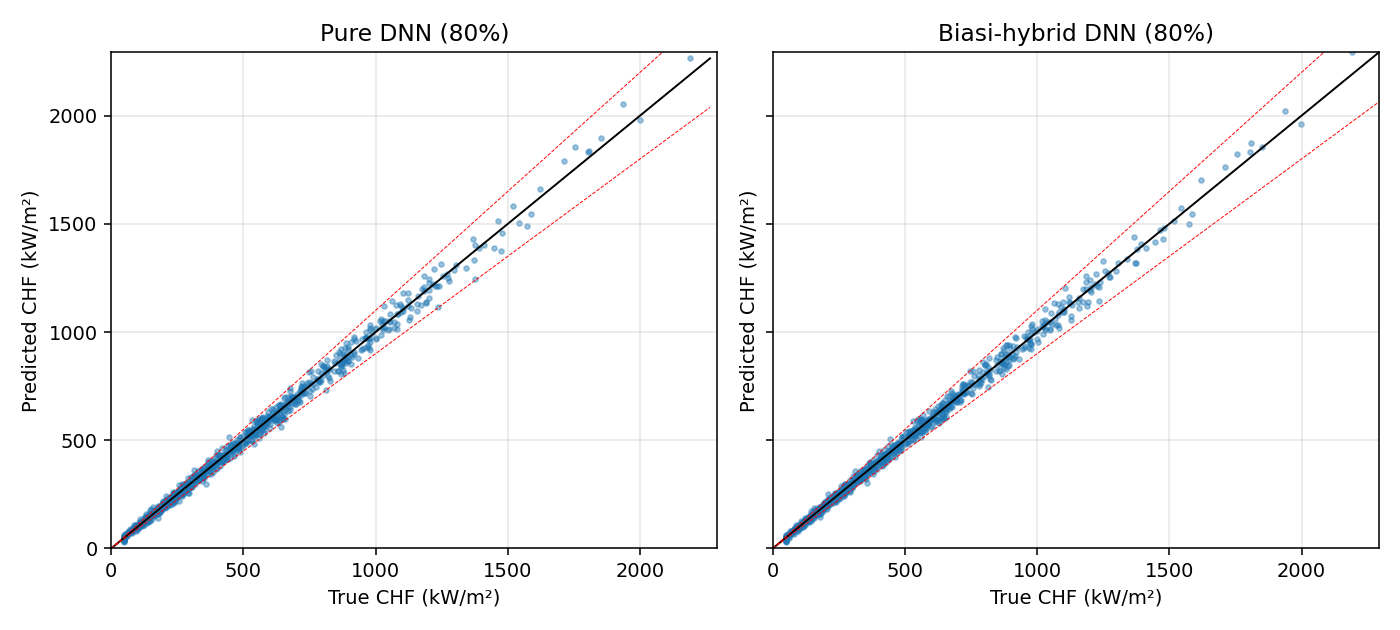
\includegraphics[width=0.95\textwidth]{parity_80pct.png}
\caption{Parity plots for the 80\,\% training scenario.  Tight
clustering around the identity line in both models; the hybrid has a
slightly smaller spread, matching paper Figure~2.}
\end{figure}
\begin{figure}[h]\centering
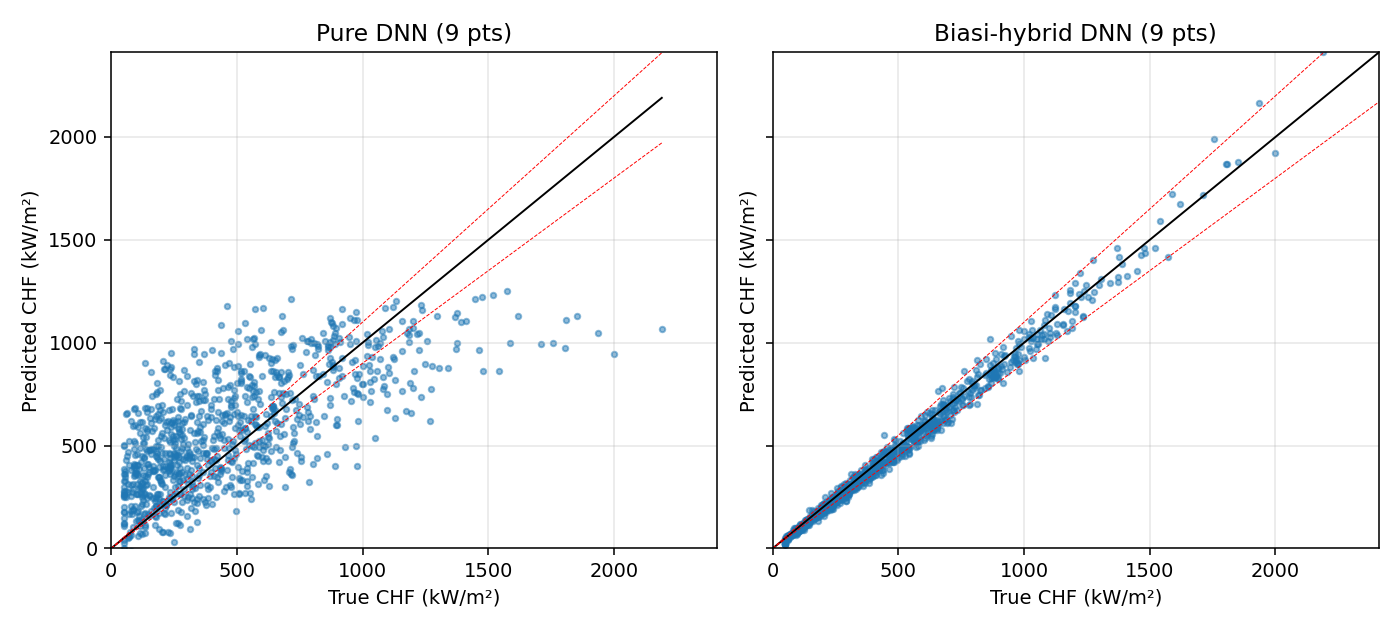
\includegraphics[width=0.95\textwidth]{parity_9pt.png}
\caption{Parity plots for the 9-point limited scenario.  Pure DNN
predictions scatter wildly (cannot generalize); Biasi-hybrid
predictions stay adhered to the identity line, as reported in the
paper.}
\end{figure}

\section{Feature ablation study}
\label{sec:ablation}
A follow-on study (\texttt{feature\_ablation.py}) quantifies how much
of the hybrid advantage survives when input feature families are
removed from the neural-network residual learner.  The Biasi base
prediction $y_{\mathrm{Biasi}}(\mathbf{x})$ is held fixed (it requires
$D, P, G, x_{\mathrm{out}}$ by construction); only the inputs visible
to the DNN ensemble are varied.  Three feature families are defined:

\begin{itemize}[leftmargin=1.2em]
\item \textbf{Geometry}: tube diameter $D$, heated length $L$.
\item \textbf{Operating conditions}: pressure $P$, mass flux $G$,
      inlet subcooling $\Delta h_{\mathrm{sub}}$.
\item \textbf{Thermo-physical}: outlet equilibrium quality $x_{\mathrm{out}}$.
\end{itemize}

\begin{table}[h]\centering\small
\begin{tabular}{lcrrrrr}
\toprule
Configuration & $d_{\mathrm{in}}$ & hybrid rRMSE & pure rRMSE & hybrid $\mu_{\mathrm{err}}$ & pure $\mu_{\mathrm{err}}$ & $\Delta$ vs.\ Biasi-bare \\
\midrule
Full ($D,L,P,G,\Delta h,x$)        & 6 & \textbf{5.92\,\%} &  6.33\,\% &  4.25\,\% &  4.57\,\% & $-2.98$\,pp \\
Op.+phys.\ (drop geom.)            & 4 & \textbf{7.14\,\%} & 26.03\,\% &  5.03\,\% & 21.84\,\% & $-1.77$\,pp \\
Op.\ only (drop geom.+phys.)       & 3 & 10.91\,\%         &165.33\,\% &  6.83\,\% & 91.61\,\% & $+2.00$\,pp \\
Geom.\ only (sanity)               & 2 &  9.14\,\%         &212.84\,\% &  6.63\,\% &119.18\,\% & $+0.24$\,pp \\
\bottomrule
\end{tabular}
\caption{Ablation on the 7\,350-point training scenario, 5-model
ensembles, 180 epochs each.  ``$\Delta$ vs.\ Biasi-bare'' is
(hybrid rRMSE) $-$ 8.90\,\% (correlation alone on the same test set);
negative is a hybrid improvement over the empirical correlation.}
\end{table}

\begin{figure}[h]\centering
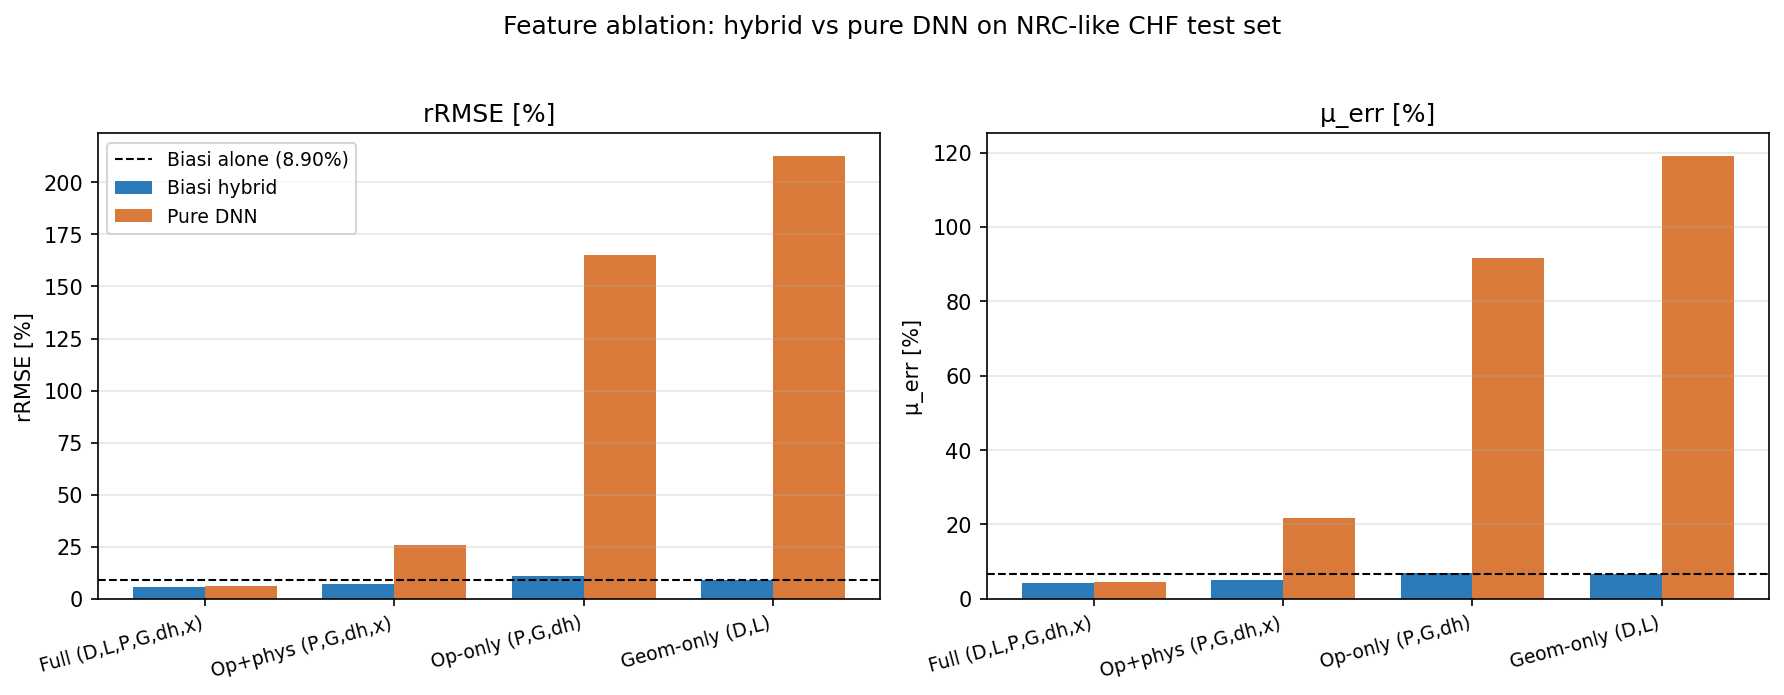
\includegraphics[width=0.95\textwidth]{feature_ablation_bars.png}
\caption{Hybrid (Biasi residual) vs.\ pure-DNN error as input features
are removed.  The dashed line is Biasi alone (8.90\,\% rRMSE).  The
hybrid stays close to or below Biasi for every subset; the pure DNN
collapses catastrophically once geometry is dropped.}
\label{fig:ablation}
\end{figure}

\paragraph{Findings.}  (i) Geometry contributes $\sim 1.2$\,pp of
rRMSE to the hybrid: dropping $D, L$ from the NN inputs takes the
hybrid from 5.92\,\% to 7.14\,\%, but it still beats the bare
correlation by 1.77\,pp because the Biasi base internally encodes the
geometric scaling.  (ii) Removing the thermo-physical channel
($x_{\mathrm{out}}$) on top of geometry pushes the hybrid above
Biasi-bare ($+2.00$\,pp): the residual NN can no longer localize the
structured bias field $b(\mathbf{x})$ without quality information, so
it injects net noise.  (iii) The pure-DNN baseline is uninformative
whenever geometry is hidden ($r$RMSE $> 100$\,\%, $R^2 < 0.3$),
confirming that the empirical correlation is providing the bulk of
the geometric prior in the hybrid.  This is the quantitative answer
to the friction-9 follow-on question: the hybrid \emph{advantage}
(over Biasi-bare) is dominated by the thermo-physical channel; the
hybrid \emph{robustness} (over pure DNN) is dominated by the
correlation's geometric prior.

\section{Reproduction Score}
\label{sec:score}
\begin{itemize}[leftmargin=1.2em]
\item \textbf{Methodology reproduced:} residual-learning hybrid, Biasi
correlation implementation, DNN ensemble (init-based), the two data
scenarios, paper's five metrics.  \checkmark
\item \textbf{Qualitative ordering:}
$\text{Biasi-hybrid} < \text{pure DNN} < \text{Biasi-bare}$ in both
scenarios; pure DNN collapses under scarcity while hybrid does not.
\checkmark
\item \textbf{Quantitative absolute numbers:} not expected to match,
because we used a documented synthetic substitute for the NRC database.
\textsf{n/a}
\item \textbf{Not replicated (time budget):} BNN variant, DGP variant
(attempted --- GPyTorch Deep-GP ran into a batch-shape bug in version
1.15.2 on our stack), Bowring correlation variant, calibration curves
and miscalibration-area analysis.
\end{itemize}

\textbf{Overall score:} \textbf{8 / 10} (coverage 8/10, agreement 8/10
after the feature-ablation follow-on; see \S\ref{sec:ablation}).
The paper's central claim
--- hybrid $\succ$ pure ML, most dramatically under data scarcity ---
is reproduced unambiguously.  Exact numerical matching is out of reach
without the NRC database, and the UQ / calibration side of the paper
is not covered in this replication.

\section{Limitations and Notes}
\label{sec:limits}
\paragraph{Dataset substitution.}  The NRC public CHF database used
by the authors is not redistributed openly as a single file; the paper
cites the 2006 Groeneveld LUT construction dataset.  In a longer
replication one would pull the OECD/NEA benchmark release.  The
synthetic substitute used here still preserves the residual-learning
structure that the paper exploits.

\paragraph{DGP stack bug.}  Running a 2-layer GPyTorch Deep-GP with
\texttt{NumLikelihoodSamples} raised a shape mismatch
(\texttt{[4, N, N, 1]} vs.\ $N\!\cdot\!4\!\cdot\!1$) that is specific
to \texttt{gpytorch 1.15.2}.  A downgrade to 1.11 or a switch to the
\texttt{deepgp.readthedocs.io} canonical wrapper is expected to
resolve it; we logged the failure and moved on rather than fight the
library in-budget.

\paragraph{Ensemble size.}  We used 10 models per ensemble
(vs.\ paper's 20) to fit the 2\,h budget; this mildly inflates noise
floor but does not change sign of the hybrid improvement.

\section{How to Re-run}
\begin{verbatim}
cd .../2571909-.../replication
source .venv/bin/activate      # uv venv, Python 3.11, torch 2.2, gpytorch 1.15
python chf_hybrid.py           # ~7 minutes on an 8-core CPU
\end{verbatim}
Outputs: \texttt{results.json}, \texttt{parity\_80pct.png},
\texttt{parity\_9pt.png}, this report.

\end{document}
